\section{Introduzione}
\subsection{Contesto Applicativo}
\begin{frame}{Convenzione}
  \begin{columns}[t]
    \begin{column}{0.45\textwidth}
      \begin{flushleft}
	\vskip2ex
	... un accordo fra l'Università ed una azienda per la realizzazione di un prodotto.
      \end{flushleft}
      \end{column}
     \begin{column}{0.55\textwidth}
      \begin{figure}[h]
	\centering
	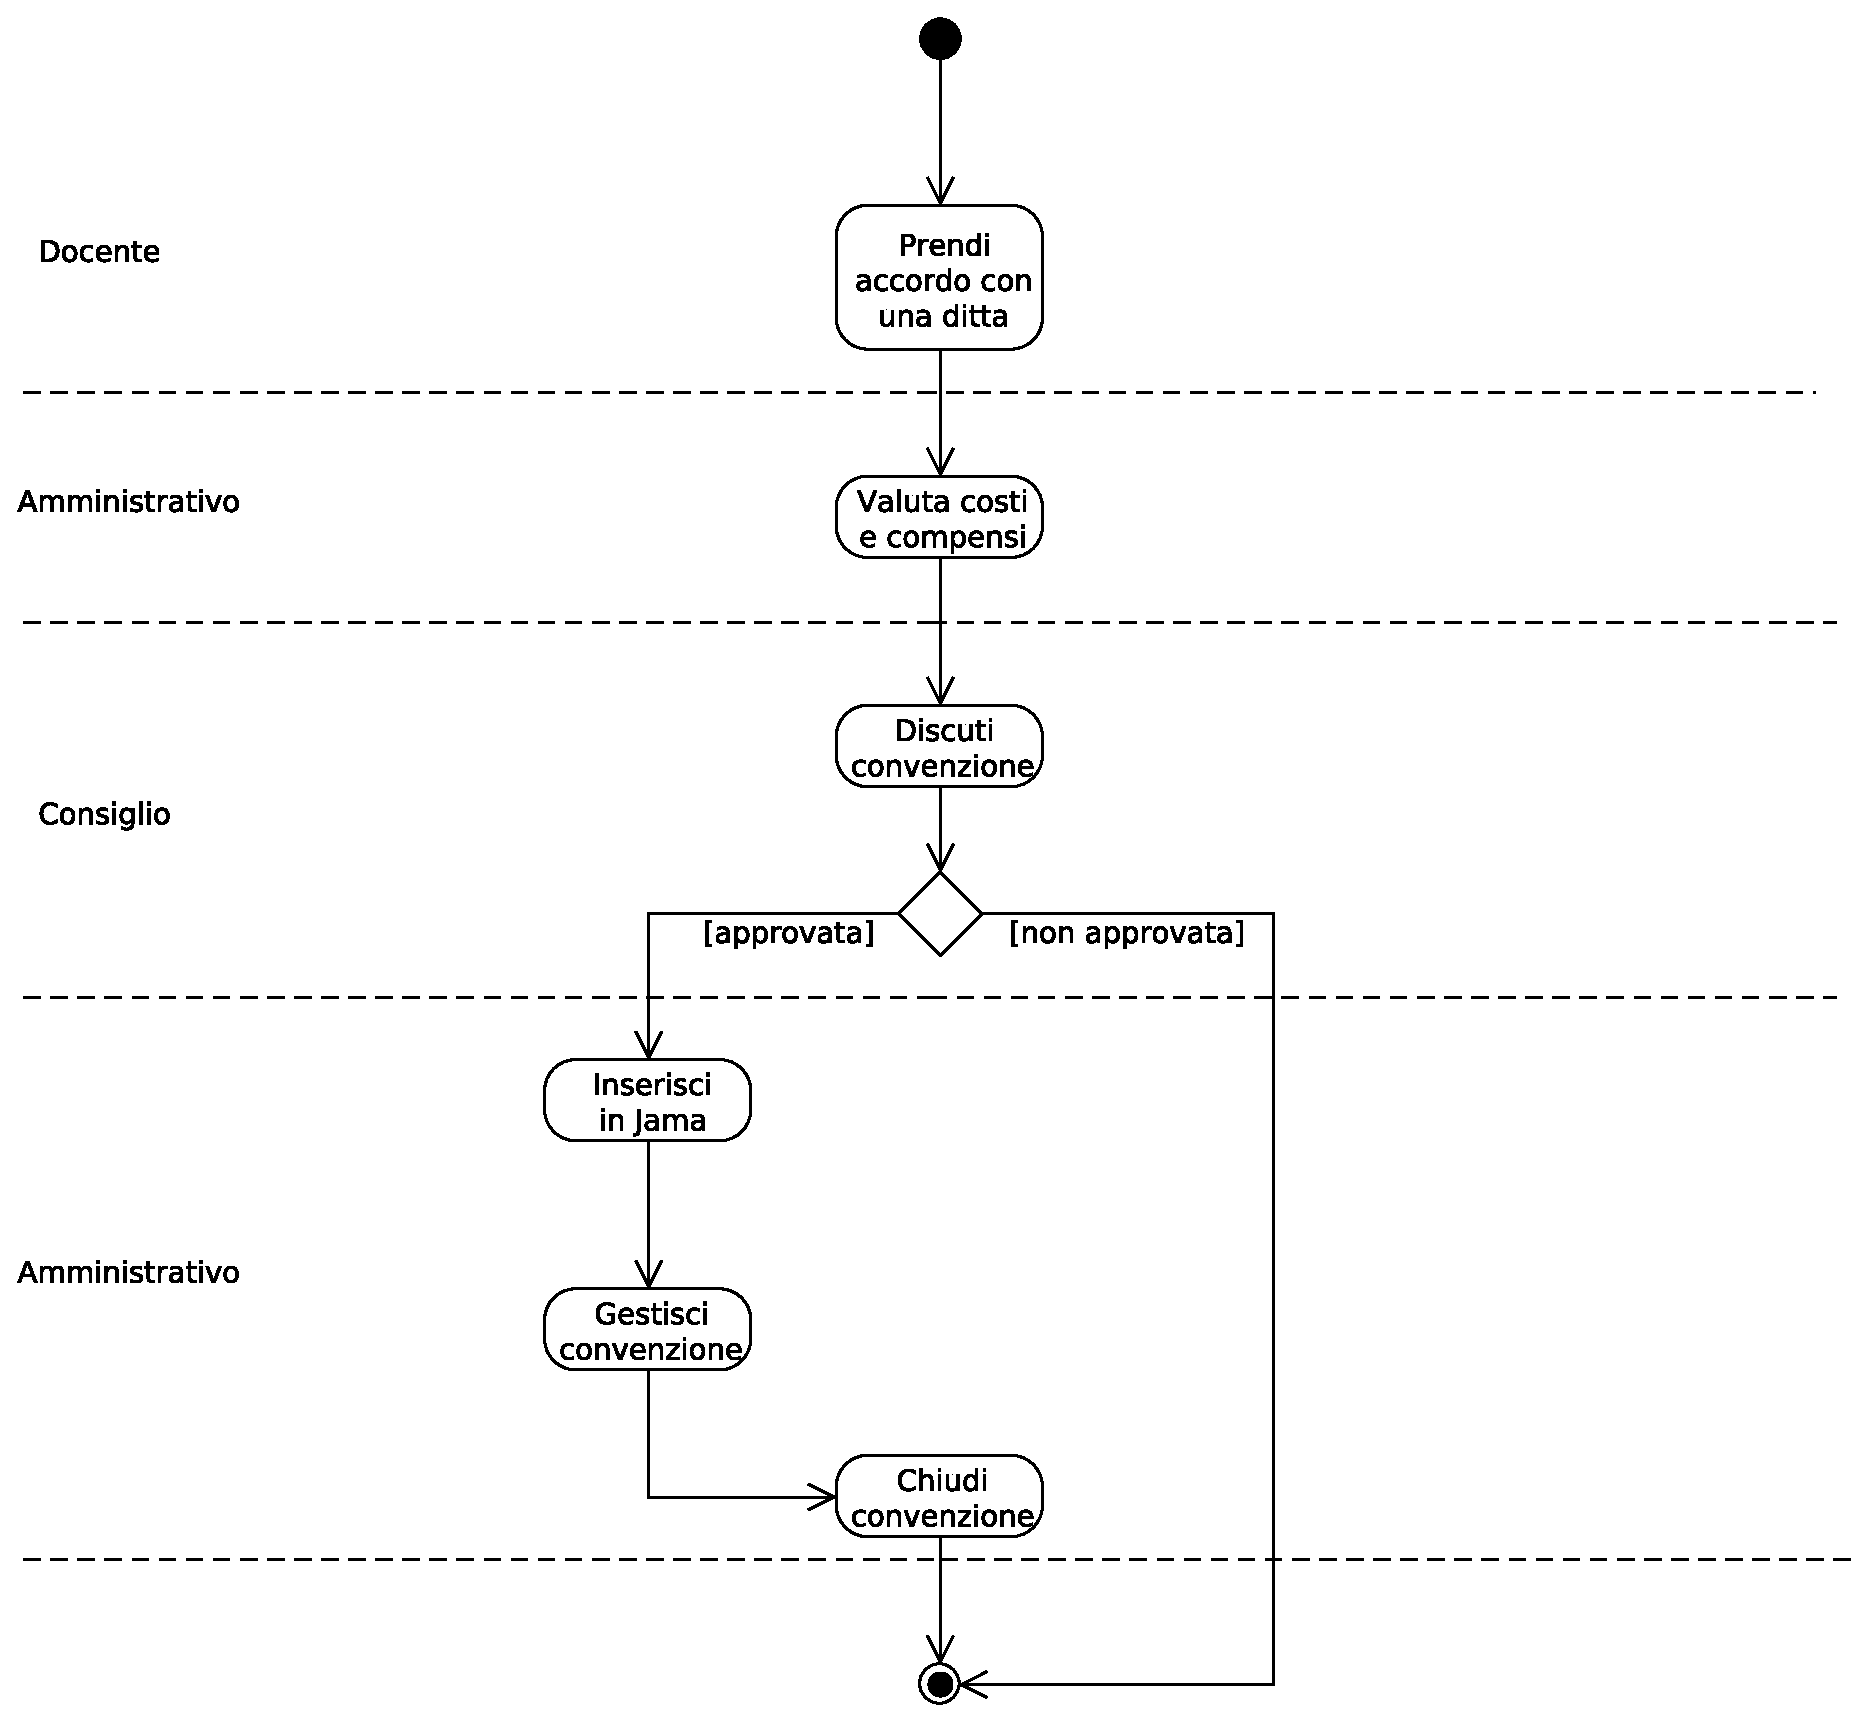
\includegraphics[scale=0.2]{images/convenzione_activity_diag.eps}
      \end{figure}
     \end{column}
\end{columns}
 
\end{frame}

\subsection{Requisiti}
\begin{frame}{Requisiti principali}
  \vskip-3ex
  L'applicazione deve consentire di:\\
  \vskip3ex
  \begin{itemize}
   \item inserire convenzioni
   \item inserire rate per una convenzione
   \item visualizzare le convenzioni inserite
   \item aggiornare i dati di una convenzione
   \item notificare le scadenze
  \end{itemize}

\end{frame}

\section{Analisi}
  \begin{frame}{Agenti}
    \begin{columns}[t]
      \begin{column}{0.7\textwidth}
    \vskip-3ex
    \begin{itemize}
     \item L'Operatore amministrativo:\\
     \vskip2ex
      \begin{itemize}
       \item inserisce, modifica convenzioni
       \item inserisce le rate
      \end{itemize}
     \vskip2ex
     \item Il Docente:\\
      \begin{itemize}
       \item visualizza lo stato delle proprie convenzioni
      \end{itemize}
     \vskip2ex
     \item Il Tempo:\\
      \begin{itemize}
       \item notifica le scadenze
      \end{itemize}
      \vskip2ex
      \item Amministratore
	\begin{itemize}
	 \item Gestisce gli utenti e i loro ruoli
	\end{itemize}

     \end{itemize}
    \end{column}
    \begin{column}{0.3\textwidth}
      \vskip-3em
     \begin{figure}[h]
	\centering
	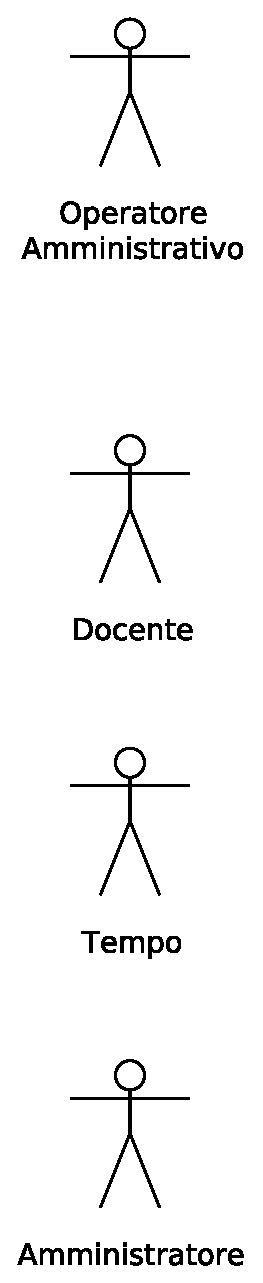
\includegraphics[scale=0.3]{images/agenti.eps}
      \end{figure}
    \end{column}


    \end{columns}
  \end{frame}

  \subsection{Casi d'Uso}
  \begin{frame}{Casi d'uso dell'Operatore amministrativo}
    \begin{figure}[h]
    \label{use_case_diag_operator}
    \centering
    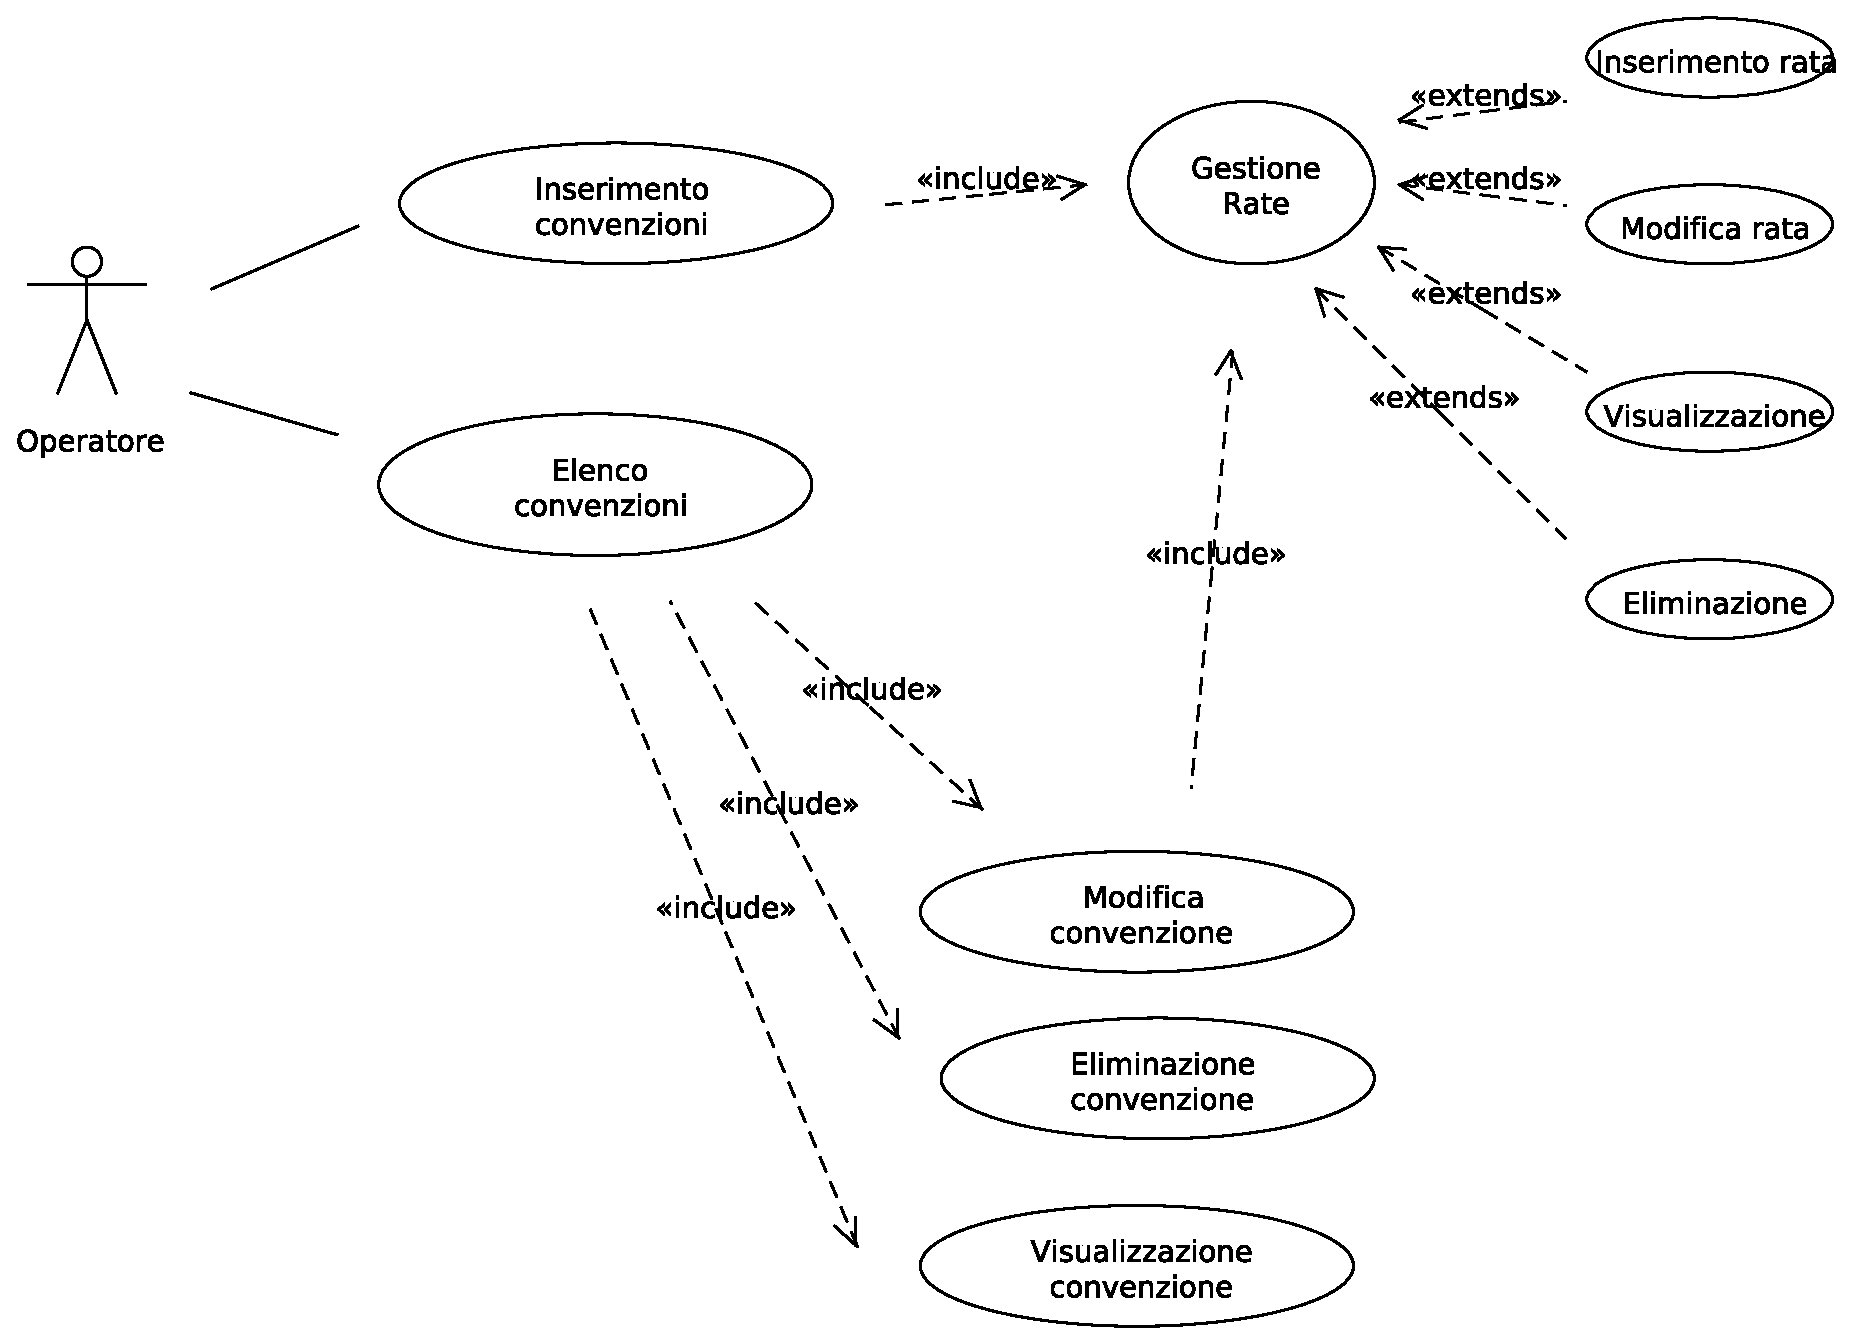
\includegraphics[height=0.85\textheight, width=0.75\textwidth]{images/casi_uso_operatore_semplified.eps}
    \end{figure}
  \end{frame}
  
   \begin{frame}{Esempio di caso d'uso}
\tiny
    \begin{tabular}{| l | l|}
      \hline
       \textbf{UC \#D1} & \textbf{Inserisci convenzione} \\
      \hline
      Level & User goal \\
      \hline
      Actor & Operatore Amministrativo \\
      \hline
      Preconditions & L'Operatore deve aver effettuato il login \\
	\hline
      Basic Course & {\tiny
	\begin{minipage}{0.7\textwidth}
	  \vskip1ex
	  \begin{enumerate}
	    \item l'Operatore clicca su ``Crea una convenzione"; viene visualizzata una schermata suddivisa in varie schede,
	      ognuna corrispondente ad un passo della procedura.
	    \item inserisce i dati della convenzione : il titolo, l'importo totale, la data di approvazione, la ditta, \ldots
	    \item inserisce la tabella di ripartizione
	    \item inserisce delle rate  
	    \item inserisce la documentazione relativa alla convenzione
	    \item clicca su ``Salva," la convenzione viene salvata e la procedura termina. Si ritorna alla schermata precedente. 
	\end{enumerate}
	\vskip1ex
	
      \end{minipage}
      }
      \\
      \hline
      Alternative courses & {\tiny
	\begin{minipage}{0.7\textwidth}
	\vskip1ex
	\begin{itemize}
	 \item [xa]   l'Operatore clicca sul tasto ``Salva'' o ``Successivo'' senza aver compilato alcuni dei campi obbligatori, o avendo inserito dei valori non consentiti; viene visualizzato un messaggio di errore 
	    e il documento non viene salvato. La schermata non viene cambiata, dando la possibilità all'Operatore di procedere alla correzione.
	 \item[xb]   durante uno qualsiasi dei passi, l'Operatore  clicca sul tasto ``Annulla'', che comporta, a seguito di una conferma, il ritorno alla schermata precedente
	    senza che la convenzione venga inserita o i cambiamenti effettuati salvati.\\
	\end{itemize}

  
  \vskip1ex


  \vskip1ex
	\end{minipage}
	}
\\
      \hline
    \end{tabular}
   \end{frame}

  
  \begin{frame}{}
    \begin{columns}[t]
      \begin{column}{0.4\textwidth}
      
      
      
      
    \tiny
    \begin{tabular}{| l | l|}
      \hline
       \textbf{UC \#D1} & \textbf{Inserisci convenzione} \\
      \hline
      Level & User goal \\
      \hline
      Actor & Operatore Amministrativo \\
      \hline
      Preconditions & L'Operatore deve aver effettuato il login \\
	\hline
      Basic Course & {\tiny
	\begin{minipage}{0.7\textwidth}
	  \vskip1ex
	  \begin{enumerate}
	    \item l'Operatore clicca su ``Crea una convenzione"; viene visualizzata una schermata suddivisa in varie schede,
	      ognuna corrispondente ad un passo della procedura.
	    \item \ldots 
	\end{enumerate}
	\vskip1ex
	
      \end{minipage}
      }
      \\
      \hline
      Alternative courses & {\tiny
	\begin{minipage}{0.6\textwidth}
	\vskip1ex
	\begin{itemize}
	 \item [xa]   l'Operatore clicca sul tasto ``Salva'' o ``Successivo'' senza aver compilato alcuni dei campi \ldots \\
	 \item[xb]   durante uno qualsiasi dei passi, l'Operatore  clicca sul tasto ``Annulla'' \ldots \\
	\end{itemize}

  
  \vskip1ex


  \vskip1ex
	\end{minipage}
	}
\\
      \hline
    \end{tabular}
      \end{column}
      \begin{column}{0.7\textwidth}
	\vskip5ex
       \begin{figure}[h]
        \centering
        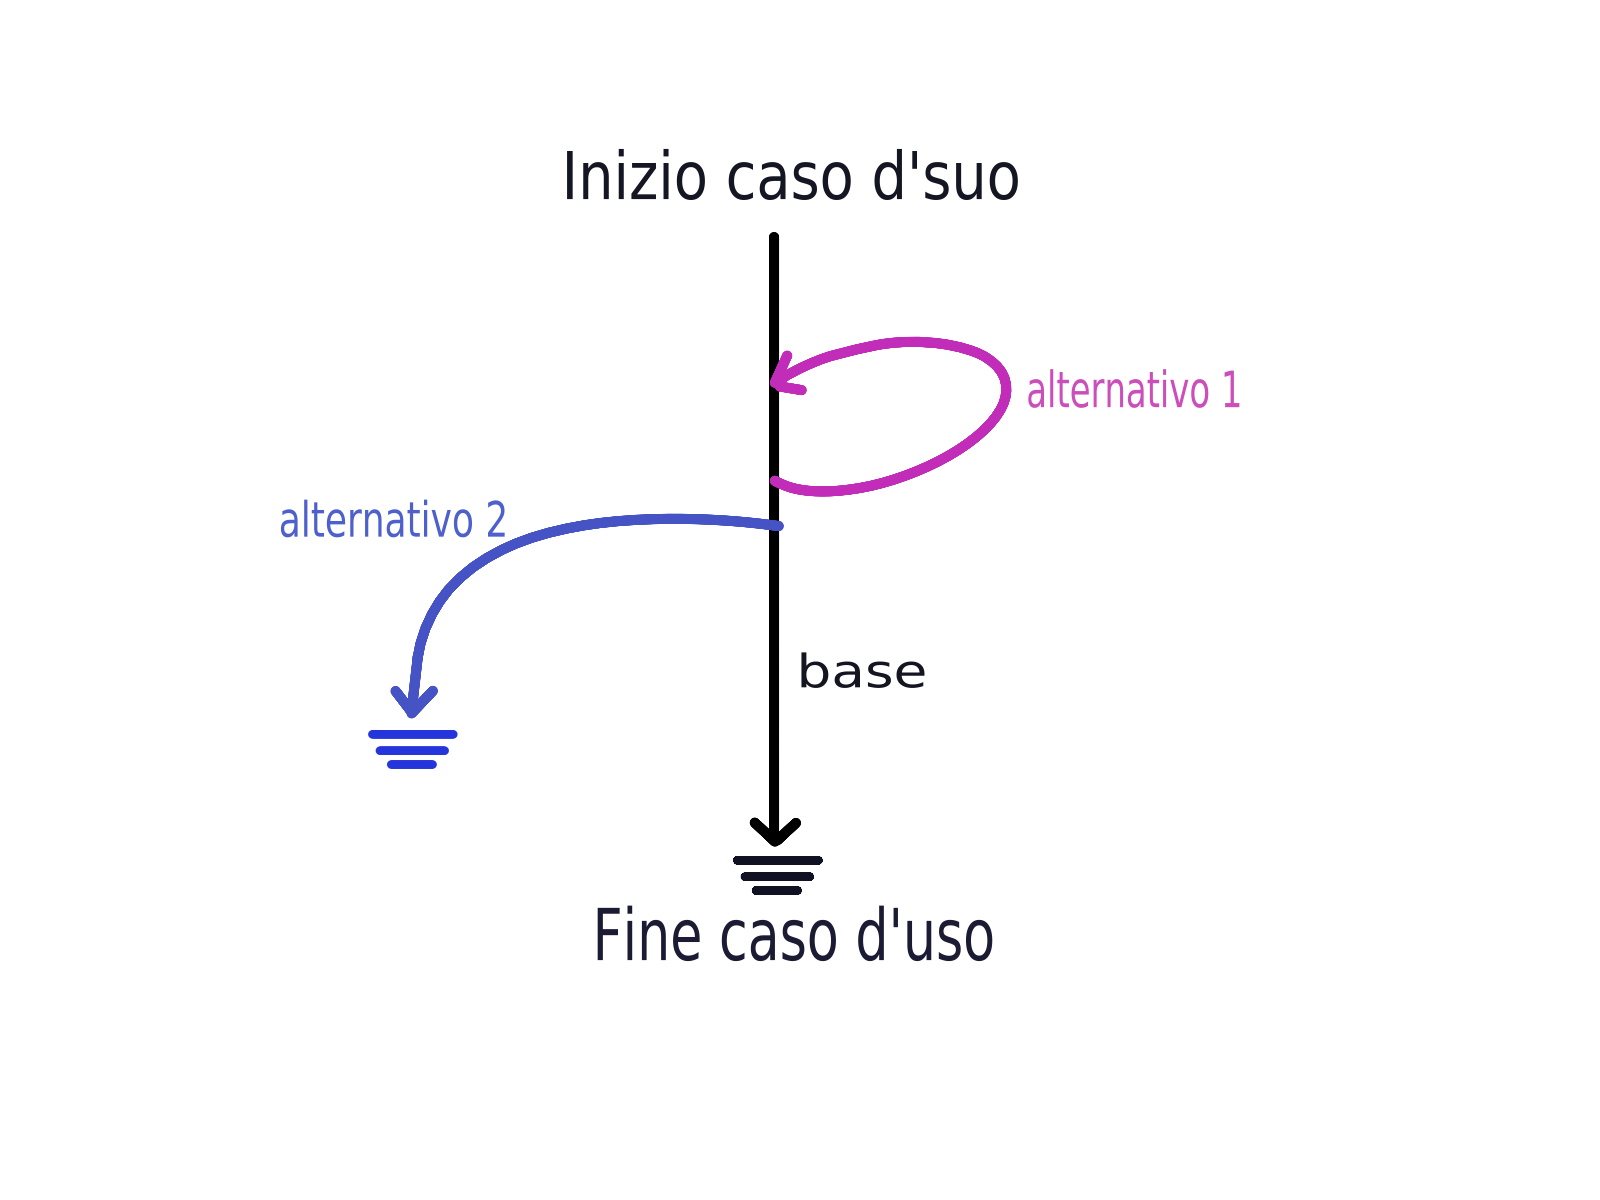
\includegraphics[scale=0.15]{images/flows.png}
       \end{figure}
      \end{column}
     \end{columns}
    \end{frame}


  
  \begin{frame}{Casi d'uso del Docente}
    \begin{figure}[h]
      \label{use_case_diag_teacher}
      \centering
      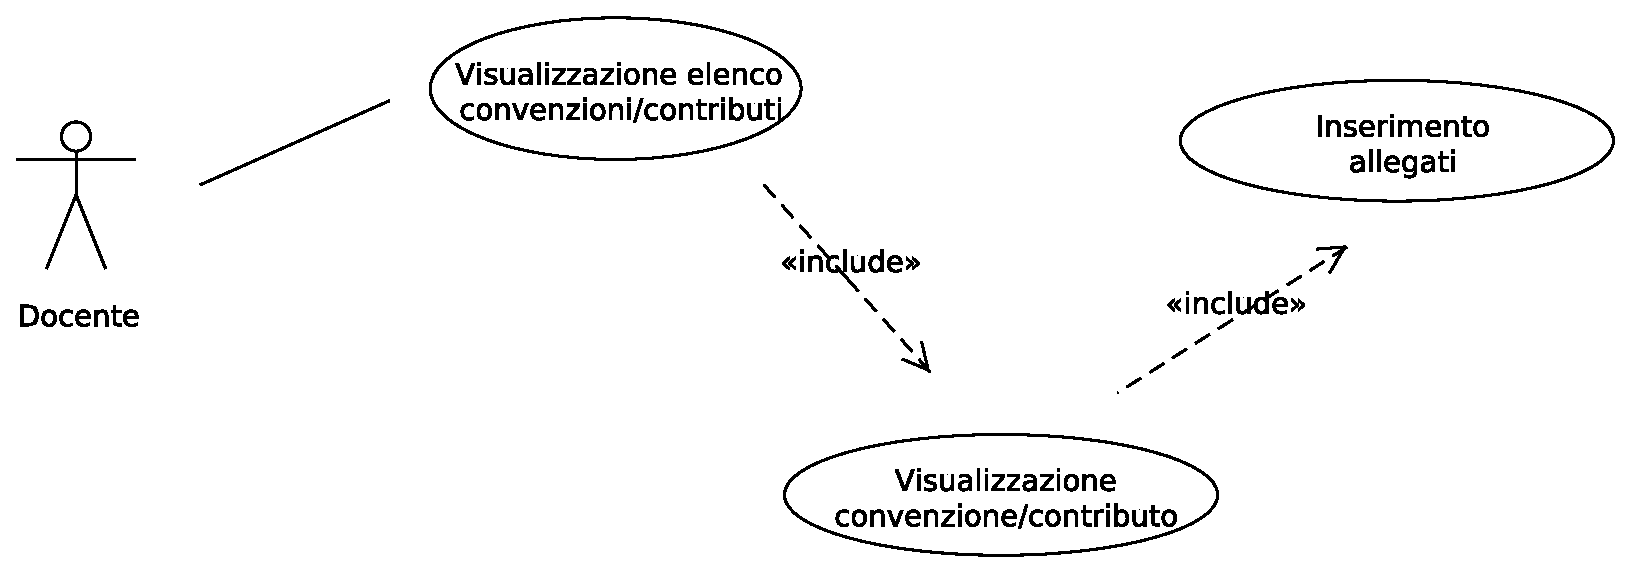
\includegraphics[width=0.5\textwidth]{images/casi_uso_docente.eps}
    \end{figure}
  \end{frame}
  
  \begin{frame}{Casi d'uso del Tempo}
    \begin{figure}[h]
      \label{use_case_diag_time}
      \centering
      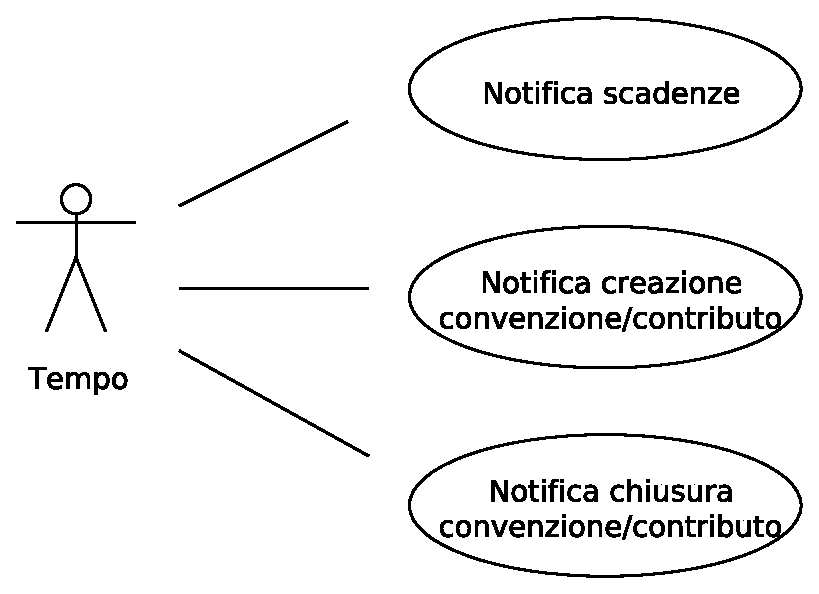
\includegraphics[width = 0.4\textwidth]{images/casi_uso_tempo.eps}
    \end{figure}
  \end{frame}
  
  \begin{frame}{Caso d'uso dell'Amministratore}
    \begin{figure}
     \centering
           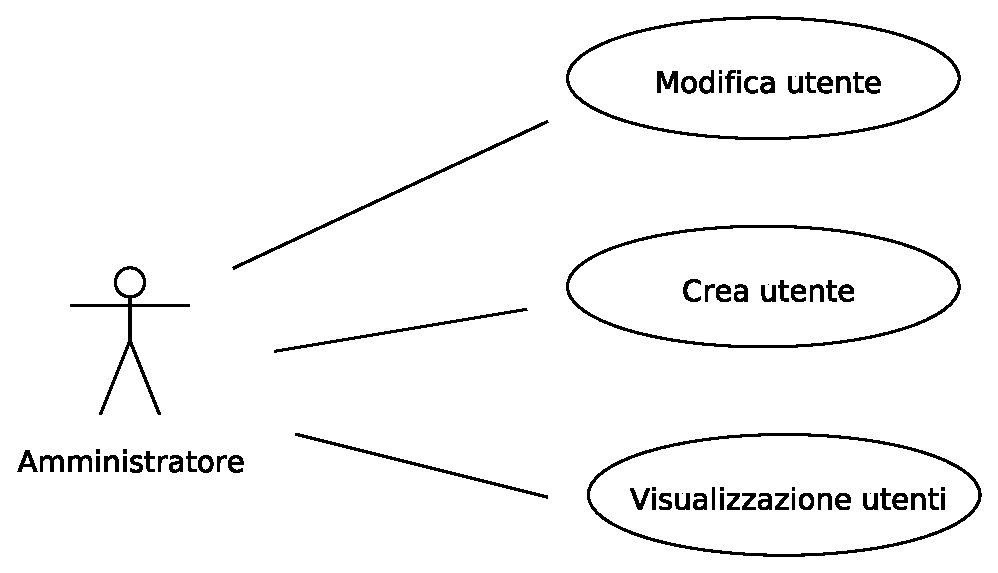
\includegraphics[width = 0.5\textwidth]{images/casi_uso_amministratore.eps}
    \end{figure}

  \end{frame}



  
  \subsection{Modello di Business}
  \begin{frame}{Modello di Dominio}
     \begin{itemize}
      \item Convenzione
      \item Rata
      \item Responsabile Scientifico
      \item Ditta
      \item ...
     \end{itemize}

   
  \end{frame}
  
  \begin{frame}{Diagramma delle classi}
  
    \begin{figure}[h]
      \label{business_model}
      \centering
      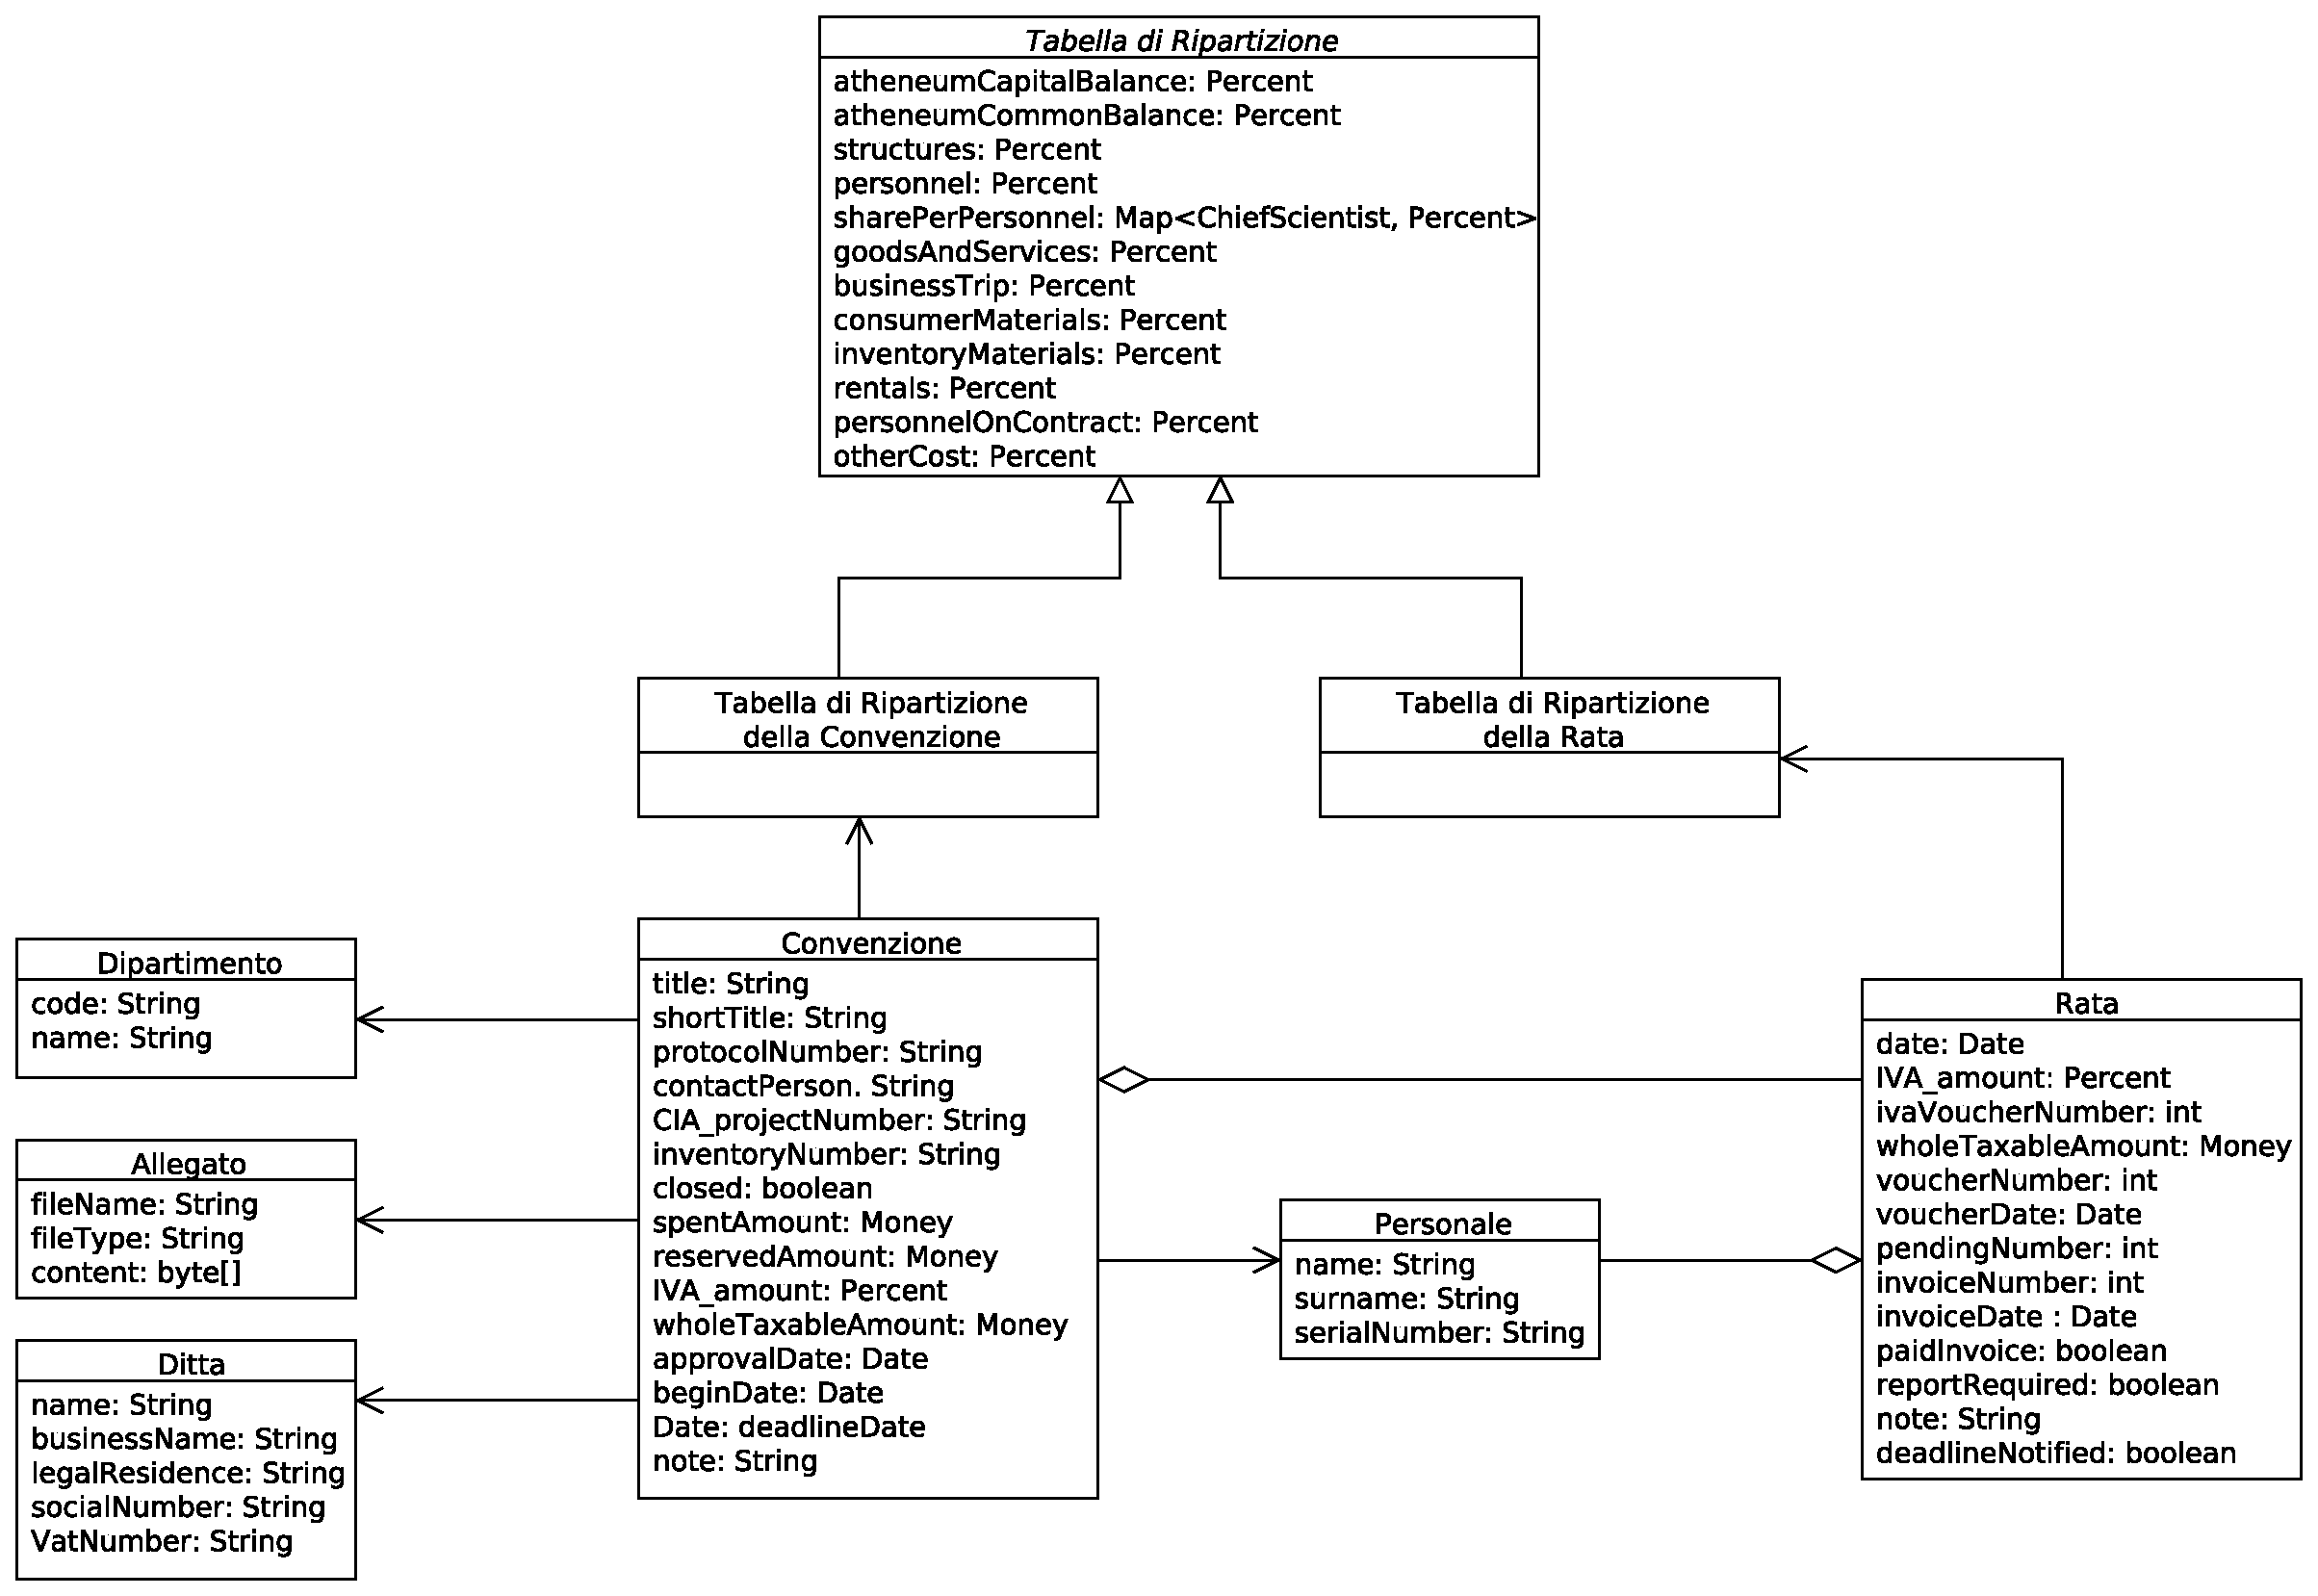
\includegraphics[width=0.9\textwidth]{images/modello_business_simplified.eps}
    \end{figure}
   
  \end{frame}


  
  



